%%%%%%%%%%%%%%%%%%%%%%%%%%%%%%%%%%%%%%%%%
% Structured General Purpose Assignment
% LaTeX Template
%
% Template Name: Anthony
% The template was named after my friend Anthony.
% Strong inspired by Apache Hadoop and Java (programming language)
%
% Author: Ang LEE
%
% Blog: http://angli.me/
%
% Github: https://github.com/leeang/
%
%%%%%%%%%%%%%%%%%%%%%%%%%%%%%%%%%%%%%%%%%

%----------------------------------------------------------------------------------------
%	CONSTANTS
%----------------------------------------------------------------------------------------

\newcommand{\hmwkTitle}{Report\ \#3}					% Assignment title
\newcommand{\hmwkClass}{Signal Processing}				% Course name
\newcommand{\hmwkClassTime}{}							% Workshop time
\newcommand{\hmwkClassInstructor}{}						% Tutor name
\newcommand{\hmwkAuthorName}{Ang LEE}					% Student name

\newcommand{\hmwkGraphicsPath}{img/}					% Graphics path
\newcommand{\hmwkCodePath}{code}						% Code path

%----------------------------------------------------------------------------------------
%	TEMPLATE
%----------------------------------------------------------------------------------------

\documentclass{article}

\usepackage{fancyhdr}	% Required for custom headers
\usepackage{lastpage}	% Required to determine the last page for the footer
\usepackage{extramarks} % Required for headers and footers
\usepackage{graphicx}	% Required to insert images
\graphicspath{\hmwkGraphicsPath}
\usepackage{lipsum} 	% Used for inserting dummy 'Lorem ipsum' text into the template

\usepackage{epstopdf}	% Required to insert .eps images
\usepackage{amssymb}
\usepackage{amsmath}
\DeclareMathOperator{\DFT}{DFT}
\DeclareMathOperator{\IDFT}{IDFT}
\usepackage[hidelinks]{hyperref}

% MATLAB syntax highlighting
\usepackage{color}		% Required to define colors
\definecolor{commentColor}{RGB}{34,139,34}
\definecolor{stringColor}{RGB}{160,32,240}
\usepackage{listings}
\lstset{
	inputpath=\hmwkCodePath,
	language=Matlab,
	basicstyle=\footnotesize\ttfamily,
	keywordstyle=\color{blue},
	stringstyle=\color{stringColor},
	commentstyle=\usefont{T1}{pcr}{m}{n}\color{commentColor},
	breaklines=true,
	showstringspaces=false,
	numbers=left,
	numberstyle=\scriptsize,
	firstnumber=1,
	numberfirstline=true,
	stepnumber=5,
	frame=leftline
}

\usepackage{fontspec}
\setmonofont{Lucida_Console.ttf}
\setsansfont[BoldFont=Lucida_Grande_Bold.ttf]{Lucida_Grande.ttf}
\usepackage{float}

% change \textbf textbf
\definecolor{bfcolor}{RGB}{221,75,57}
\DeclareTextFontCommand{\textbf}{\bfseries\color{bfcolor}}

% change \texttt color
\definecolor{ttcolor}{RGB}{0,103,179}
\DeclareTextFontCommand{\texttt}{\ttfamily\color{ttcolor}}

% change headings color
\usepackage{sectsty}
\definecolor{sectioncolor}{RGB}{0,102,33}
\sectionfont{\color{sectioncolor}\sffamily}
\definecolor{subsectioncolor}{RGB}{26,131,171}
\subsectionfont{\color{subsectioncolor}\sffamily}
\definecolor{subsubsectioncolor}{RGB}{0,51,102}
\subsubsectionfont{\color{subsubsectioncolor}\sffamily}

% Margins
\topmargin=-0.45in
\evensidemargin=-0.3in
\oddsidemargin=-0.3in
\textwidth=7.1in
\textheight=9.0in
\headsep=0.25in

\linespread{1.1}		% Line spacing

% Set up the header and footer
\pagestyle{fancy}
\lhead{\hmwkTitle} % Header Left 
\chead{\hmwkAuthorName} % Header Center
\rhead{\hmwkClass} % Header Right
\lfoot{\url{https://github.com/leeang/Signal-Processing}} % Footer Left
\cfoot{} % Footer Center
\rfoot{Page\ \thepage\ of\ \pageref{LastPage}} % Footer Right
\renewcommand\headrulewidth{0.4pt} % Size of the header rule
\renewcommand\footrulewidth{0.4pt} % Size of the footer rule

\setlength\parindent{0pt} % Removes all indentation from paragraphs

%----------------------------------------------------------------------------------------
%	Problem and Section
%----------------------------------------------------------------------------------------

\newenvironment{homeworkProblem}[1]{
	\section*{#1}
	}{
}
\newenvironment{homeworkSection}[1]{
	\subsection*{#1}
	}{
}
\newcommand{\problemAnswer}[1]{
	\noindent\framebox[\columnwidth][c]{
		\begin{minipage}{0.98\columnwidth}
			#1
		\end{minipage}
	}
}

%----------------------------------------------------------------------------------------
%	Document
%----------------------------------------------------------------------------------------

\begin{document}

\newpage

%----------------------------------------------------------------------------------------
%	PROBLEM
%----------------------------------------------------------------------------------------

\begin{homeworkProblem}{Part A Question 1}

%--------------------------------------------

\begin{homeworkSection}{(a)}

The overlap-add method is an efficient way to evaluate the discrete convolution of a very long signal $x[n]$ of length $L_0$ with a FIR filter $h[n]$ of length $M$.

\begin{equation}
h[n] =
\begin{cases}
b_k & k = 0, 1, \cdots, M-1\\
0 & \text{otherwise}\\ 
\end{cases}
\end{equation}

The covlution
\begin{equation}
y[n] = \sum_{k=0}^{M-1} h[k]x[n-k] = h[0]x[n] + h[1]x[n-1] + \cdots + h[M-1]x[n-M+1]
\end{equation}
has length $L_0+M-1$, i.e. $y[n]=0$ for $n<0$ and $n \ge L_0+M-1$.\\

The concept is to divide the problem into multiple convolutions of $h[n]$ with short segments of $x[n]$:
\begin{equation}
x_k[n] :=
\begin{cases}
x[n+(k-1)L] & n=0, 1, \cdots, L-1\\
0 & n= L, L+1, \cdots, N-1
\end{cases}
\end{equation}
where $L$ is an arbitrary segment length and $k=1, 2, 3, \cdots$.
\begin{equation}
x[n] = \sum_{k} x_k[n-(k-1)L]
\end{equation}
$y[n]$ can be written as a sum of short convolutions:
\begin{equation}
y[n] = \left( \sum_{k} x_k[n-(k-1)L] \right) * h[n] = \sum_{k} x_k[n-(k-1)L] * h[n] = \sum_{k} y_k[n-(k-1)L]
\end{equation}
where $y_k[n] := x_k[n] * h[n]$ is zero for $n<0$ and $n \ge L+M-1$. And for any parameter $N\ge L+M-1$, it is equivalent to the $N$-point circular convolution of $x_k[n]$, with $h[n]$, in the region $[0, N-1]$.\\

Reference: \url{https://en.wikipedia.org/wiki/Overlap%E2%80%93add_method}

\end{homeworkSection}

%--------------------------------------------

\end{homeworkProblem}

%----------------------------------------------------------------------------------------
%	PROBLEM
%----------------------------------------------------------------------------------------

\begin{homeworkProblem}{Part A Question 2}

%--------------------------------------------

\begin{homeworkSection}{(a)}

\begin{equation}
X[k] = \DFT\{x[m]\} = \sum_{m=0}^{N-1} x[m] W_{N}^{km}
\end{equation}

\begin{align*}
y[n] &= \DFT\{X[k]\}\\
&= \sum_{k=0}^{N-1} X[k] W_{N}^{kn}\\
&= \sum_{k=0}^{N-1} \sum_{m=0}^{N-1} x[m] W_{N}^{km} W_{N}^{kn}\\
&= \sum_{k=0}^{N-1} x[m] \sum_{m=0}^{N-1} W_{N}^{k(m+n)}
\end{align*}

Considering that $(m+n) \in [0, 2N-2]$,
\begin{equation}
\sum_{m=0}^{N-1} W_{N}^{k(m+n)} = \sum_{m=0}^{N-1} e^{\frac{-j 2\pi}{N} k(m+n)} =
\begin{cases}
N & m = N-n\\
0 & \text{otherwise}\\ 
\end{cases}
\end{equation}

Therefore,
\begin{equation}
y[n] = N \cdot x[N-n]
\end{equation}

\subsubsection*{Algorithm}
\begin{equation}
X[k] \xrightarrow{\text{FFT}} y[n] \xrightarrow{\text{divided by N}} x[N-n] \xrightarrow{\text{flip}} x[n+1] \xrightarrow{\text{right shift by 1}} x[n]
\end{equation}

\begin{table}[!hbp]
\centering
\begin{tabular}{c c c c c c c c}
$y[n]$ &$y[0]$ &$y[1]$ &$y[2]$ &$\cdots$ &$y[N-3]$ &$y[N-2]$ &$y[N-1]$ \\
divided by N &$x[0]$ &$x[N-1]$ &x$[N-2]$ &$\cdots$ &$x[3]$ &$x[2]$ &$x[1]$ \\
flip &$x[1]$ &$x[2]$ &x$[3]$ &$\cdots$ &$x[N-2]$ &$x[N-1]$ &$x[0]$ \\
right shift by 1 &$x[0]$ &$x[1]$ &x$[2]$ &$\cdots$ &$x[N-3]$ &$x[N-2]$ &$x[N-1]$ \\
\end{tabular}
\caption{algorithm deduction}
\end{table}

\end{homeworkSection}

%--------------------------------------------

\end{homeworkProblem}

%----------------------------------------------------------------------------------------
%	PROBLEM
%----------------------------------------------------------------------------------------

\begin{homeworkProblem}{Part A Question 3}

%--------------------------------------------

\begin{homeworkSection}{(a)}

\begin{equation}\label{A3a1}
X[k] = X^*[\langle-k\rangle_{2N}] = X^*[2N-k]
\end{equation}

\begin{align*}
X[k] &= \sum_{n=0}^{N-1} x[n] e^{-j \frac{2 \pi kn}{2N} }\\
X[2N-k] &= \sum_{n=0}^{N-1} x[n] e^{-j \frac{2 \pi (2N-k) n}{2N} }\\
X^*[2N-k] &= \sum_{n=0}^{N-1} x^*[n] e^{j \frac{2 \pi (2N-k) n}{2N} }\\
&= \sum_{n=0}^{N-1} x^*[n] e^{j 2 \pi n} e^{-j \frac{2 \pi kn}{2N} }\\
&= \sum_{n=0}^{N-1} x^*[n] e^{-j \frac{2 \pi kn}{2N}}
\end{align*}
Note that: $(z+w)^* = z^* + w^*$, $(zw)^* = z^* w^*$\\

Substituting into $X[k] = X^*[2N-k]$ (Eq. \ref{A3a1}) yields
\begin{equation}
\sum_{n=0}^{N-1} x[n] e^{-j \frac{2 \pi kn}{2N} } = \sum_{n=0}^{N-1} x^*[n] e^{-j \frac{2 \pi kn}{2N}}\\
\end{equation}
Therefore, $x[n] = x^*[n]$, i.e. $x[n]=\IDFT\{X[k]\}$ is real.

\end{homeworkSection}

%--------------------------------------------

\begin{homeworkSection}{(b)}

\begin{align*}
X_0[k] &= X[k] + X[k+N]\\
&= X^*[2N-k] + X^*[2N-(k+N)]\\
&= X^*[2N-k] + X^*[N-k]\\
&= X^*[N-k] + X^*[(N-k)+N]\\
&= X_0^*[N-k]
\end{align*}
Hence, $X_0[k]$ is conjugate symmetric.

\begin{align*}
j X_1[k] &= W_{2N}^{-k} (X[k] - X[k+N])\\
&= j W_{2N}^{-k} (X^*[2N-k] - X^*[2N-(k+N)])\\
&= j W_{2N}^{-k} (X^*[2N-k] - X^*[N-k])\\
&= j W_{2N}^{-k} (X^*[N-k] - X^*[(N-k)+N])\\
&= j X_1^*[N-k]\\
&= - (j)^* X_1^*[N-k]\\
&= - (j X_1[N-k])^*\\
&= - (j X_1[\langle-k\rangle_N])^*
\end{align*}
Hence, $jX_1[k]$ is conjugate anti-symmetric.

\end{homeworkSection}

%--------------------------------------------

\begin{homeworkSection}{(c)}

Calculate $q[n]$
\begin{align*}
q[n] &= \IDFT\{Q[k]\} = \frac{1}{N} \sum_{k=0}^{N-1} (X_0[k] + j X_1[k]) e^{j \frac{2 \pi n}{N} k}\\
&= \frac{1}{N} \sum_{k=0}^{N-1} \left(X[k] + X[k+N] + j W_{2N}^{-k} X[k] - j W_{2N}^{-k} X[k+N]\right) e^{j \frac{2 \pi n}{N} k}\\
&= \frac{1}{N} \sum_{k=0}^{N-1} \left(X[k] (1 + j W_{2N}^{-k}) + X[k+N] (1 - j W_{2N}^{-k})\right) e^{j \frac{2 \pi n}{N} k}\\
&= \frac{1}{N} \sum_{k=0}^{N-1} \left(X[k] (1 + j W_{2N}^{-k}) + X[k+N] (1 - j W_{2N}^{-k})\right) e^{j \frac{2 \pi n}{N} k}\\
&= \frac{1}{N} \sum_{k=0}^{N-1} \left(X[k] (1 + j W_{2N}^{-k})\right) e^{j \frac{2 \pi n}{N} k} + \frac{1}{N} \sum_{k=0}^{N-1} \left(X[k+N] (1 - j W_{2N}^{-k})\right) e^{j \frac{2 \pi n}{N} k}\\
&= \frac{1}{N} \sum_{k=0}^{N-1} \left(X[k] (1 + j W_{2N}^{-k})\right) e^{j \frac{2 \pi n}{N} k} + \frac{1}{N} \sum_{k=N}^{2N-1} \left(X[k] (1 - j W_{2N}^{-(k-N)})\right) e^{j \frac{2 \pi n}{N} (k-N)}\\
&= \frac{1}{N} \sum_{k=0}^{N-1} \left(X[k] (1 + j W_{2N}^{-k})\right) e^{j \frac{2 \pi n}{N} k} + \frac{1}{N} \sum_{k=N}^{2N-1} \left(X[k] (1 + j W_{2N}^{-k})\right) e^{j \frac{2 \pi n}{N} k} e^{- j 2\pi n}\\
&= \frac{1}{N} \sum_{k=0}^{2N-1} \left(X[k] (1 + j W_{2N}^{-k})\right) e^{j \frac{2 \pi n}{N} k}
\end{align*}
Note that: $- W_{2N}^{-(k-N)} = - (e^{-j \frac{2\pi}{2N}})^{-(k-N)} = - e^{j \frac{\pi (k-N)}{N}} = e^{j \frac{\pi (k-N)}{N} + j\pi} = e^{j \frac{\pi k}{N}} = W_{2N}^{-k}$\\

Calculate $q^*[n]$
\begin{align*}
q^*[n] &= \frac{1}{N} \sum_{k=0}^{2N-1} \left(X^*[k] (1 - j W_{2N}^{k})\right) e^{-j \frac{2 \pi n}{N} k}\\
&= \frac{1}{N} \sum_{k=0}^{2N-1} \left(X[2N-k] (1 - j W_{2N}^{k})\right) e^{-j \frac{2 \pi n}{N} k}\\
&= \frac{1}{N} \sum_{k=1}^{2N} \left(X[k] (1 - j W_{2N}^{2N-k})\right) e^{-j \frac{2 \pi n}{N} (2N-k)}\\
&= \frac{1}{N} \sum_{k=1}^{2N} \left(X[k] (1 - j W_{2N}^{-k})\right) e^{-j 4 \pi n} e^{j \frac{2 \pi n}{N} k}\\
&= \frac{1}{N} \sum_{k=1}^{2N-1} \left(X[k] (1 - j W_{2N}^{-k})\right) e^{j \frac{2 \pi n}{N} k} + X[2N] (1 - j)\\
&= \frac{1}{N} \sum_{k=1}^{2N-1} \left(X[k] (1 - j W_{2N}^{-k})\right) e^{j \frac{2 \pi n}{N} k} + X[0] (1 - j)\\
&= \frac{1}{N} \sum_{k=0}^{2N-1} \left(X[k] (1 - j W_{2N}^{-k})\right) e^{j \frac{2 \pi n}{N} k}
\end{align*}
Note that: $W_{2N}^{2N-k} = (e^{-j \frac{2\pi}{2N}})^{2N-k} = e^{-j2\pi} (e^{-j\frac{2\pi}{2N}})^{-k} = W_{2N}^{-k}$\\

$x[2n]$ and $x[2n+1]$ can be expressed in terms of $q[n]$ and $q^*[n]$.
\begin{equation}
\frac{1}{2} \Re\{q[n]\} = \frac{1}{4} (q[n] + q^*[n])
= \frac{1}{2N} \sum_{k=0}^{2N-1} X[k] e^{j \frac{2 \pi n}{N} k}
= \frac{1}{2N} \sum_{k=0}^{2N-1} X[k] W_{2N}^{-2nk}
= x[2n]
\end{equation}
\begin{equation}
\frac{1}{2} \Im\{q[n]\} = \frac{1}{4j} (q[n] - q^*[n])
= \frac{1}{2N} \sum_{k=0}^{2N-1} X[k] W_{2N}^{-k} e^{j \frac{2 \pi n}{N} k}
= \frac{1}{2N} \sum_{k=0}^{2N-1} X[k] W_{2N}^{-(2n+1)k}
= x[2n+1]
\end{equation}

Q.E.D.

\end{homeworkSection}

%--------------------------------------------

\begin{homeworkSection}{(d)}

1. Constitute $X_0[k] = X[k] + X[k+N]$ and $X_1[k] = W_{2n}{-k}(X[k] - X[k+N])$ ($k = 0, \cdots N-1$)\\
2. Constitute $Q[k] = X_0[k] + jX_1[k]$\\
3. Compute $N$-point IDFT of $Q[k]$\\
4. $x[2n] = \frac{1}{2} \Re\{q[n]\}$ and $x[2n+1] = \frac{1}{2} \Im\{q[n]\}$

\end{homeworkSection}

%--------------------------------------------

\begin{homeworkSection}{(e)}

The advantage of overlap add method is that the circular convolution can be computed very efficiently as follows, according to the circular convolution theorem:
\begin{equation}
y[n] = \IDFT\Big(\DFT(x[n])\cdot\DFT(h[n])\Big)
\end{equation}
where DFT and IDFT refer to the discrete Fourier transform and inverse discrete Fourier transform, respectively, evaluated over $N$ discrete points.

\subsubsection*{Radix-2 FFT}
Each butterfly requires:\\
\textbf{one} complex multiplication\\
\textbf{two} complex additions\\

In total, there are: $\frac{N}{2}$ butterflies per stage $\times$ $\log_2(N)$ stages.

%--------------------------------------------

\subsubsection*{Convolution using FFT and IFFT}
\begin{equation}
y[n] = \sum_{k=0}^{M-1} h[k]x[n-k],\ \ \ Y[k] = H[k]X[k]
\end{equation}
\begin{tabular}{l l l}
$H[k]$ &computed once and can be ignored\\
DFT of $x[n]$ &$\frac{N}{2} \log_2(N)$ multiplications &$N \log_2(N)$ additions\\
Computation of $Y[k]$ &$N$ multiplications\\
IDFT of $Y[k]$ &$\frac{N}{2} \log_2(N)$ multiplications &$N \log_2(N)$ additions\\
In total &$N \log_2(2N)$ multiplications &$2N \log_2(N)$ additions
\end{tabular}

%--------------------------------------------

\subsubsection*{Convolution using real FFT and conjugate symmetric IFFT}

%------------------

\textbf{FFT}\\
Use a $\frac{N}{2}$-point complex FFT to evaluate a $N$-point real FFT. This algorithm is shown in the appendix on page \pageref{fft_real}.\\

Complex multiplications:
\begin{equation}
\frac{N}{4} \log_2(\frac{N}{2}) + \frac{N}{2}
\end{equation}

Complex additions:
\begin{equation}
\frac{N}{2} \log_2(\frac{N}{2}) + 2N
\end{equation}

%------------------

\textbf{Computation of $Y[k] = H[k]X[k]$}\\
Due to conjugate symmetry, only $\frac{N}{2}+1$ complex multiplications need to be calculated.\\

%------------------

\textbf{IFFT}\\
Use a $\frac{N}{2}$-point general IFFT to evaluate a $N$-point conjugate symmetric IFFT. This algorithm is shown on page \pageref{ifftcs}.\\

Complex multiplications:
\begin{equation}
\frac{N}{4} \log_2(\frac{N}{2}) + \frac{N}{2}
\end{equation}

Complex additions:
\begin{equation}
\frac{N}{2} \log_2(\frac{N}{2}) + \frac{3N}{2}
\end{equation}

%------------------

\textbf{In total}\\

Complex multiplications:
\begin{equation}
\left( \frac{N}{4} \log_2(\frac{N}{2}) + \frac{N}{2} \right) \times 2 + \frac{N}{2}+1 = \frac{N}{2} \log_2(4N) + 1 \approx \frac{N}{2} \log_2(4N)
\end{equation}

Complex additions:
\begin{equation}
N \log_2(N) + 2.5N
\end{equation}

%--------------------------------------------

\subsubsection*{Complex multiplications per output data point}
\begin{equation}\label{c_nu_mlt}
c_{MLT}(\nu) = \frac{N \log_2(2N)}{L} = \frac{\frac{N}{2} \log_2(N) + N + 1}{N-M+1} = \frac{2^{\nu} (0.5\nu + 1) + 1}{2^{\nu} - M + 1}
\end{equation}

%--------------------------------------------

\subsubsection*{Complex additions per output data point}
\begin{equation}\label{c_nu_add}
c_{ADD}(\nu) = \frac{2N \log_2(N)}{L} = \frac{N \log_2(N) + 2.5N}{N-M+1} = \frac{2^{\nu} (\nu + 2.5)}{2^{\nu} - M + 1}
\end{equation}

\end{homeworkSection}

%--------------------------------------------

\end{homeworkProblem}

%----------------------------------------------------------------------------------------
%	PROBLEM
%----------------------------------------------------------------------------------------

\begin{homeworkProblem}{Part B Task 1}

%--------------------------------------------

\begin{homeworkSection}{(a)}

\subsubsection*{\texttt{iffta(X)}}
\lstinputlisting{iffta.m}

\subsubsection*{\texttt{ifftb(X)}}
\lstinputlisting{ifftb.m}

\end{homeworkSection}

%--------------------------------------------

\begin{homeworkSection}{(b)}

\begin{figure}[H]
\centering
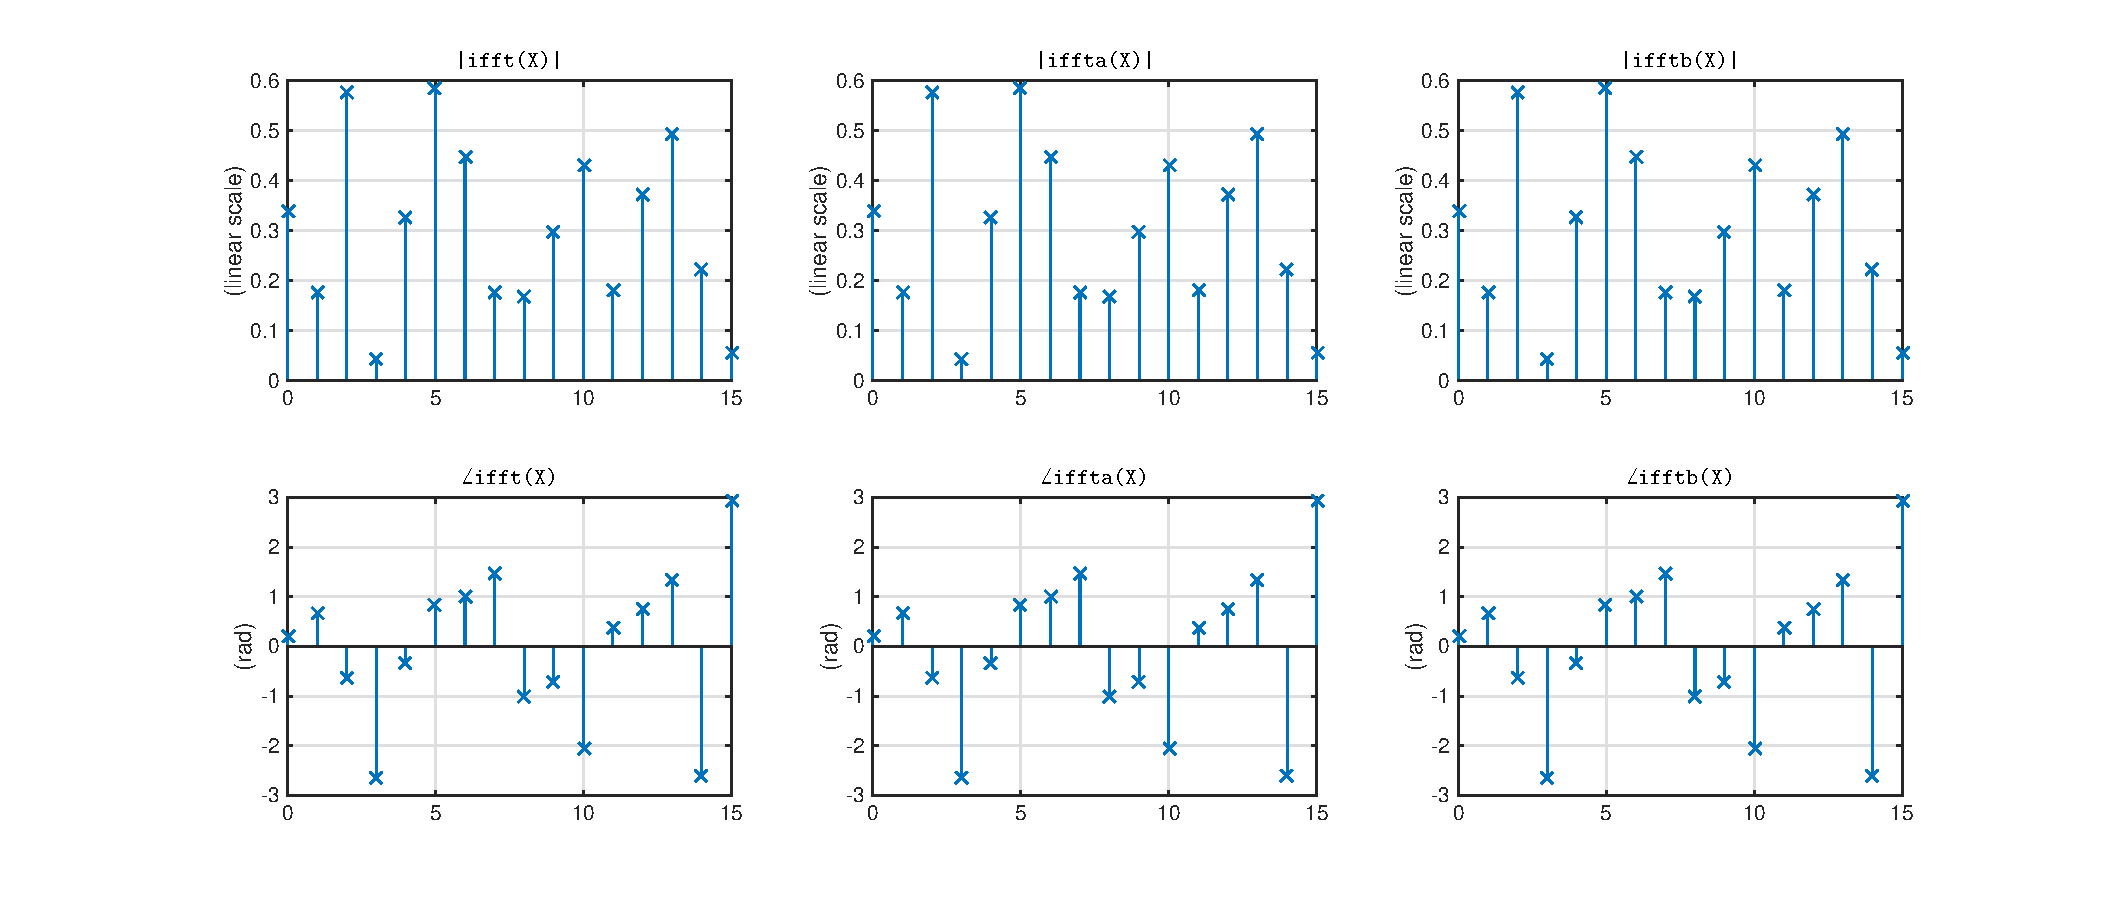
\includegraphics[width=\linewidth]{task1b}
\caption{\texttt{ifft(X)}, \texttt{iffta(X)} and \texttt{ifftb(X)}}
\label{task1b}
\end{figure}

MATLAB code can be found in Appendix on page \pageref{task1b_code}.

\end{homeworkSection}

%--------------------------------------------

\end{homeworkProblem}

%----------------------------------------------------------------------------------------
%	PROBLEM
%----------------------------------------------------------------------------------------

\newpage
\begin{homeworkProblem}{Part B Task 2}

%--------------------------------------------

\begin{homeworkSection}{(a) \texttt{isConjugateSymmetric(X)}}

\lstinputlisting{isConjugateSymmetric.m}

\end{homeworkSection}

%--------------------------------------------

\begin{homeworkSection}{(b) \texttt{ifftcs(X)}}

\lstinputlisting{ifftcs.m}\label{ifftcs}

\end{homeworkSection}

%--------------------------------------------

\begin{homeworkSection}{(c)}

\begin{figure}[H]
\begin{minipage}[t]{0.5\linewidth}
\centering
\includegraphics[width=\linewidth]{task2c1}
\caption{$|X[k]|$ and $\angle X[k]$}
\label{task2c1}
\end{minipage}
\begin{minipage}[t]{0.5\linewidth}
\centering
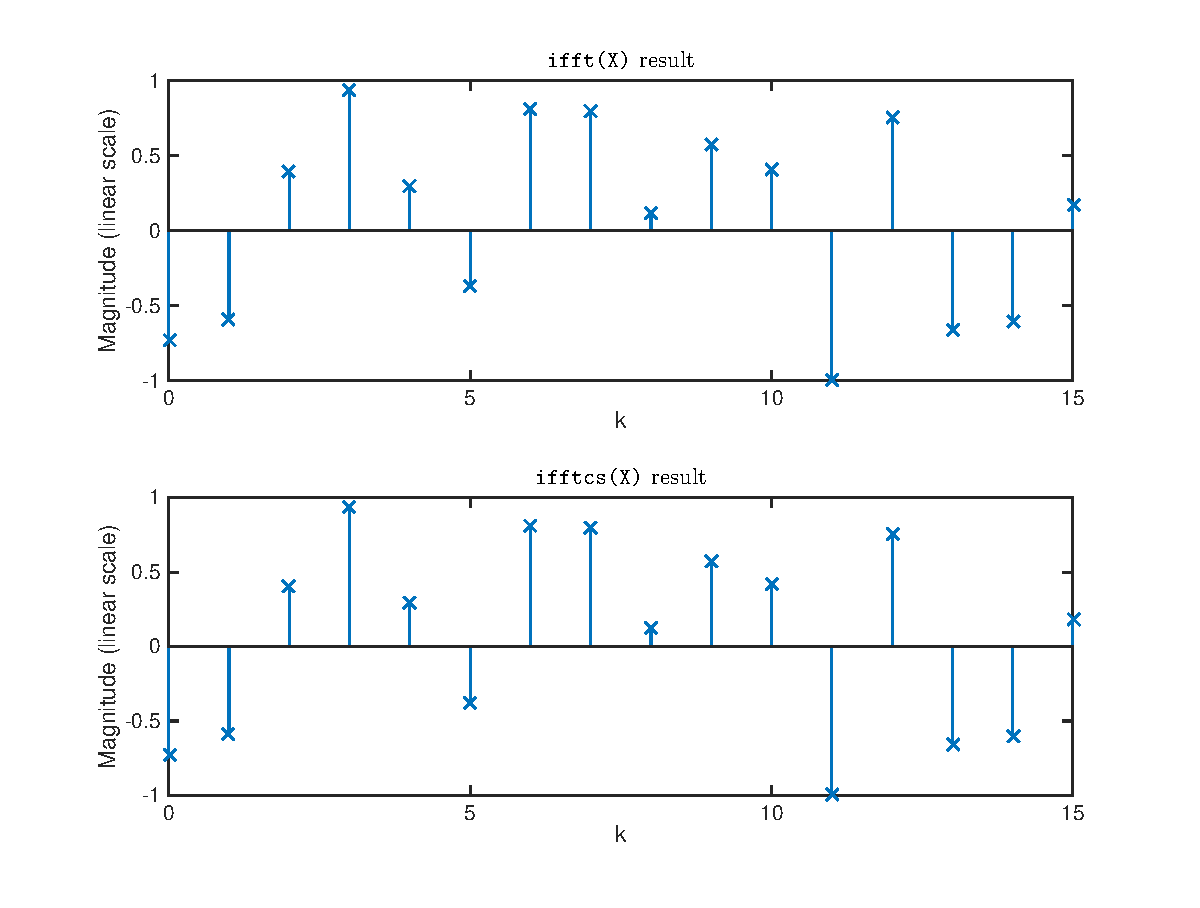
\includegraphics[width=\linewidth]{task2c2}
\caption{\texttt{ifft(X)} and \texttt{ifftcs(X)}}
\label{task2c2}
\end{minipage}
\end{figure}

MATLAB code can be found in Appendix on page \pageref{task2c_code}.

\end{homeworkSection}

%--------------------------------------------

\end{homeworkProblem}

%----------------------------------------------------------------------------------------
%	PROBLEM
%----------------------------------------------------------------------------------------

\begin{homeworkProblem}{Part B Task 3}

%--------------------------------------------

\begin{homeworkSection}{(a)}

MATLAB code can be found in Appendix on page \pageref{overlapaddreal}.

\end{homeworkSection}

%--------------------------------------------

\end{homeworkProblem}

%----------------------------------------------------------------------------------------
%	PROBLEM
%----------------------------------------------------------------------------------------

\begin{homeworkProblem}{Part B Task 4}

\textbf{MATLAB code can be found in Appendix on page \pageref{task4_code}.}

%--------------------------------------------

\begin{homeworkSection}{(a)}

The preliminary $N_{order}$ = 39 can be calculated by \texttt{firpmord(f,a,dev,fs)} function. However, the performance of the FIR filter cannot meet the design specifications, especially the stopband ripple term. We increment the filter order until all specifications are satisfied. Eventually, when \textbf{$N_{order} = 46$}, all specifications are satisfied (shown in Fig. \ref{task4a2}).\\

Thus, the length of filter response is
\begin{equation}
M = 47
\end{equation}

\begin{figure}[H]
\begin{minipage}[t]{0.5\linewidth}
\centering
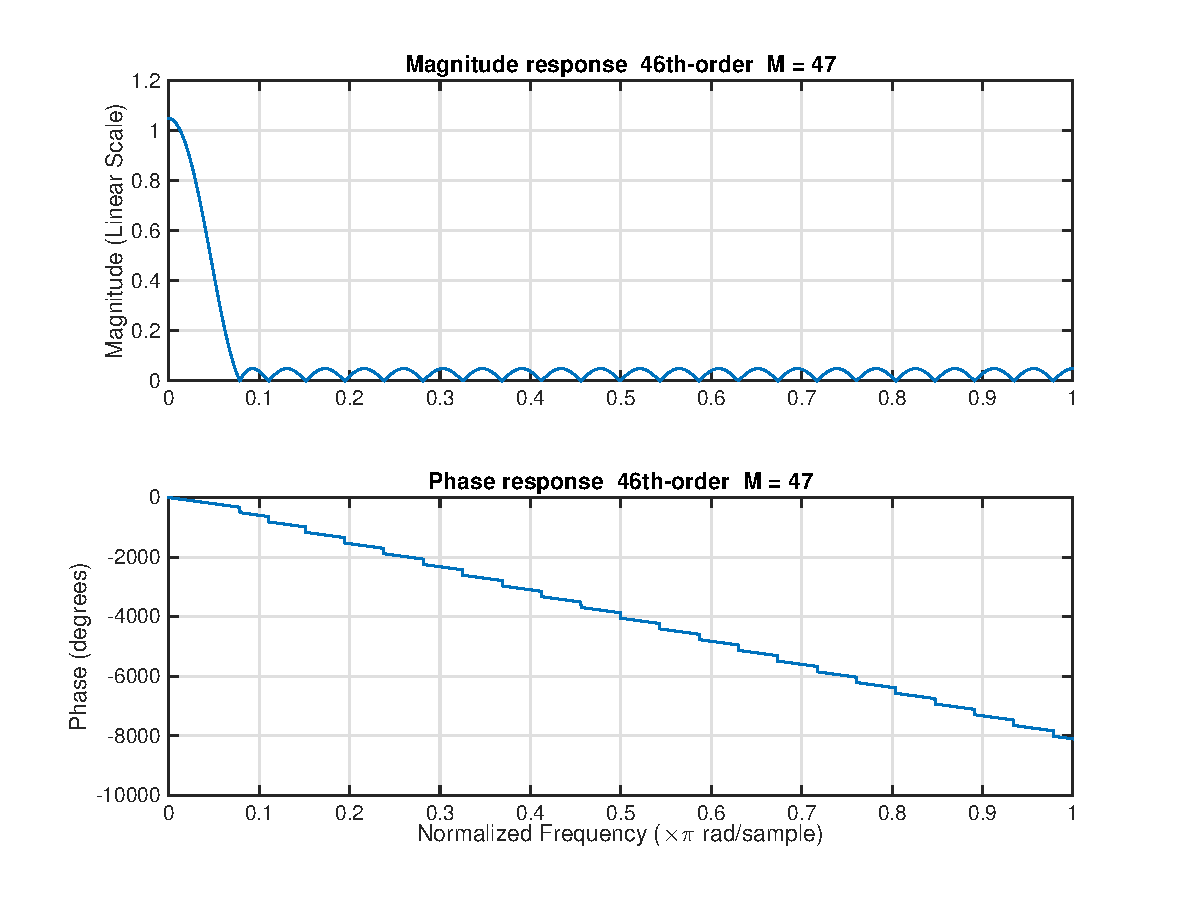
\includegraphics[width=\linewidth]{task4a1}
\caption{FIR filter frequency response}
\label{task4a1}
\end{minipage}
\begin{minipage}[t]{0.5\linewidth}
\centering
\includegraphics[width=\linewidth]{task4a2}
\caption{FIR filter frequency response (zoomed)}
\label{task4a2}
\end{minipage}
\end{figure}

\end{homeworkSection}

%--------------------------------------------

\begin{homeworkSection}{(b)}

\subsubsection*{Test signal}
\begin{figure}[H]
\begin{minipage}[t]{0.5\linewidth}
\centering
\includegraphics[width=\linewidth]{test-signal-time}
\end{minipage}
\begin{minipage}[t]{0.5\linewidth}
\centering
\includegraphics[width=\linewidth]{test-signal-frequency}
\end{minipage}
\caption{Test signal}
\label{test-signal}
\end{figure}

As is shown in Fig. \ref{test-signal}, a nine-tone sinusoid signal is designed as the test signal.
\begin{equation}
x[n] = \sum_{k=1}^{9} \sin(2\pi k f_0 n / F_s)
\end{equation}
where $f_0$ = 200 Hz.

\subsubsection*{Optimal block length}
\begin{figure}[H]
\centering
\includegraphics[width=0.5\linewidth]{computations_nu}
\caption{Relationship between $c(\nu)$ and $\nu$ for $M = 47$}
\label{computations_nu}
\end{figure}

The relationship between $c(\nu)$ and $\nu$ for $M = 47$ (Fig. \ref{computations_nu}) can be plotted based on Eq.\ref{c_nu_mlt} on page \pageref{c_nu_mlt}. It can be clear seen that, when $N = 2^9 = 512$, $c(\nu)$ reaches its minimum \textbf{$c_{MLT}(9) = 6.045$}.
\begin{equation}
N_\text{optimal} = 2^9 = 512
\end{equation}

Taking advantages of symmetry reduces \textit{complex multiplications per output data point} by
\begin{equation}
\frac{10.97 - 6.045}{10.97} \times 100\% = 45\%
\end{equation}

\subsubsection*{Output verification}
\begin{figure}[H]
\begin{minipage}[t]{0.5\linewidth}
\centering
\includegraphics[width=\linewidth]{task4b1}
\caption{Test signal and \texttt{filter} output}
\label{task4b1}
\end{minipage}
\begin{minipage}[t]{0.5\linewidth}
\centering
\includegraphics[width=\linewidth]{task4b2}
\caption{\texttt{fftfilt} output and \texttt{overlapaddreal} output}
\label{task4b2}
\end{minipage}
\end{figure}

As is shown in Fig. \ref{task4b1} and Fig. \ref{task4b2}, \texttt{filter} output, \texttt{fftfilt} output and \texttt{overlapaddreal} output are consistent. In case of any discrepancy, several lines of code are programmed to check whether outputs are accordant. If not, \textbf{warning} messages will be displayed.\\

\lstinputlisting[linerange=142-149]{task4.m}

\subsubsection*{Functions comparison}
\texttt{filter} filters data with recursive (IIR) or nonrecursive (FIR) filter. \texttt{fftfilt} filters data using the efficient FFT-based method of overlap-add, a frequency domain filtering technique that works only for \textbf{FIR} filters.\\

When the input signal is relatively large, it is advantageous to use \texttt{fftfilt} instead of \texttt{filter}, which performs $M$ multiplications for each sample in $x$, where $M$ is the filter length. \texttt{fftfilt} performs 2 FFT operations - the FFT of the signal block of length $L$ plus the inverse FT of the product of the FFTs - at the cost of $\frac{1}{2} L \log_2(L)$ where $L$ is the block length. It then performs $L$ point-wise multiplications for a total cost of $L + L \log_2(L)$ multiplications.\\

The cost ratio is therefore
\begin{equation}
\frac{\texttt{fftfilt()}}{\texttt{filter()}} = \frac{L + L \log_2(L)}{ML} = \frac{L(1 + \log_2 L)}{ML} = \frac{\log_2(2L)}{M}
\end{equation}

As a result, \texttt{fftfilt} becomes advantageous when $\log_2(2L)$ is less than $M$.\\

Reference: \url{https://www.mathworks.com/help/signal/ref/fftfilt.html}

\end{homeworkSection}

%--------------------------------------------

\begin{homeworkSection}{(c)}

\subsubsection*{\texttt{filter()}}
Complex multiplications per second
\begin{equation}
M \cdot F_s = 47 \times 24000 = 1128000
\end{equation}

Complex additions per second
\begin{equation}
(M-1) \cdot F_s = 46 \times 24000 = 1104000
\end{equation}

\subsubsection*{\texttt{fftfilt()}}
Complex multiplications per second
\begin{equation}
F_s \cdot (1 + \log_2 F_s) = 373217.9
\end{equation}

Complex additions per second
\begin{equation}
2F_s \cdot (1 + \log_2 F_s) = 746435.8
\end{equation}

\subsubsection*{Taking advantages of symmetry}
Complex multiplications per second
\begin{equation}
c(9)_{MLT} \cdot F_s = 145082
\end{equation}
$c(9)_{MLT} = 6.045$ is calculated by Eq.\ref{c_nu_mlt} on page \pageref{c_nu_mlt}.\\

Complex additions per second
\begin{equation}
c(9)_{ADD} \cdot F_s = 303245
\end{equation}
$c(9)_{ADD} = 12.63$ can be calculated by Eq.\ref{c_nu_add} on page \pageref{c_nu_add}.

\end{homeworkSection}

%--------------------------------------------

\end{homeworkProblem}

%----------------------------------------------------------------------------------------
%	PROBLEM
%----------------------------------------------------------------------------------------

\begin{homeworkProblem}{Part C}

\texttt{\_LabTasks.c} and \texttt{Params.h} can be found on page \pageref{Params_h}.\\

During the workshop session, we fed a two-tone (200Hz and 1kHz) sinusoidal signal into the DSP board. The DSP board swapped output source every 5 seconds (input, \texttt{process\_time()} output and \texttt{process\_block()} output in turn). We consider \texttt{process\_time()} and \texttt{process\_block()} functioned normally, because 1kHz-component was effectively attenuated.\\

In order to conduct a more rigorous test, we used MATLAB to generate a test signal ($\frac{24000}{200} \times 3 = 360$ points, span of three periods) and obtained the output via built-in function \texttt{filter()}. (\texttt{test.m} can be found on page \pageref{test_m}.)\\

At the next stage, we imported the test signal into a \texttt{.c} file and simulated the filtering process. \texttt{test.c} and \texttt{SPWS3.h} can be found on page \pageref{test_c}. After compiling these two files with aforementioned \texttt{\_LabTasks.c} and \texttt{Params.h}, output variables \texttt{output\_time[]} and \texttt{output\_block[]} can be inspected in ``debug perspective''.

\begin{figure}[H]
\begin{minipage}[t]{0.5\linewidth}
\centering
\includegraphics[width=\linewidth]{test_MATLAB}
\caption{MATLAB \texttt{filter()} output}
\label{test_MATLAB}
\end{minipage}
\begin{minipage}[t]{0.5\linewidth}
\centering
\includegraphics[width=\linewidth]{test_dsp}
\caption{\texttt{process\_time()} and \texttt{process\_block()}}
\label{test_dsp}
\end{minipage}
\end{figure}

As is shown in Figure \ref{test_MATLAB} and Figure \ref{test_dsp}, the outputs of \texttt{process\_time()} and \texttt{process\_block()} cannot be differentiated, and these two waveforms are consistent with the MATLAB simulation.
\end{homeworkProblem}

%----------------------------------------------------------------------------------------
%	Appendix
%----------------------------------------------------------------------------------------

\newpage
\section*{Appendix}

\subsection*{\texttt{overlapaddreal(B, x, N)}}\label{overlapaddreal}
\lstinputlisting{overlapaddreal.m}

\newpage
\subsection*{Params.h}\label{Params_h}
\lstinputlisting[language=c]{Params.h}

\subsection*{\_LabTasks.c}\label{_LabTasks}
\lstinputlisting[language=c]{_LabTasks.c}

\newpage
\subsection*{Part B Task 4}\label{task4_code}
\lstinputlisting{task4.m}

\subsection*{\texttt{fft\_real(x)}}\label{fft_real}
\lstinputlisting{fft_real.m}

\subsection*{Part B Task 1 (b)}\label{task1b_code}
\lstinputlisting{task1b.m}

\newpage
\subsection*{Part B Task 2 (c)}\label{task2c_code}
\lstinputlisting{task2c.m}

\subsection*{test.m}\label{test_m}
\lstinputlisting{test.m}

\subsection*{SPWS3.h}\label{SPWS3_h}
\lstinputlisting[language=c]{SPWS3.h}

\subsection*{test.c}\label{test_c}
\lstinputlisting[language=c]{test.c}

%----------------------------------------------------------------------------------------

\end{document}
